
\chapter{}


\section{看涨期权价差策略的介绍}
牛市价差是最流行的价差形式之一。在这类的价差交易里,投资者买入 1 手行权价的看涨期权($K_1, c_1$),同时卖出 1 手行权价更高的看涨期权($K_1, c_2$),有 $K_2>K_1, c_2<c_1$。一般来说,两手期权的到期日相同。这是一个垂直价差。当标的股票上涨时,牛市价差就会盈利,因此这是一个看多的头寸。这个价差的潜在盈利和潜在风险都是有限的。虽然两者从百分比上来看都相当可观,但风险不会超过净投资。事实上,相对于直接买入 1 手相似的看涨期权,1 手牛市价差所要求的投资金额要小一些,因此其最大潜在亏损金额也要小一些。

\begin{figure}[h]
    \centering
    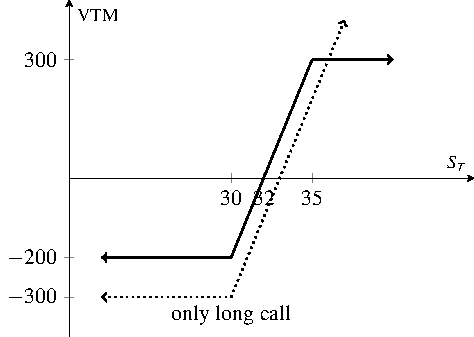
\includegraphics[width=0.7\textwidth]{IMG/call_spread_1.pdf}
    \caption{条件:$S_t=32, K_1=30, K_2=35, c_1=3, c_2=1, m=100$,到期月份为 10 月。建立这个头寸的投资者对标的股票是看多的,但是,一般而言,他是在寻找一种对冲的途径。如果他直截了当地看多,他会直接买入 10 月 30 看涨期权。而买入 10 月 30 看涨期权并卖出 10 月 35 看跌期权的交易,则让他在到期时股票价格低于 36 时的交易结果,会比直接买入 10 月 30 看涨期权要更好一些。图中的虚线显示了这一事实。}
    \label{fig:call_spread}
\end{figure}

计算一手看涨期权牛市价差的盈亏平衡点和最大潜在盈利是一件相当容易的事:
\begin{equation}
    \begin{aligned}
        B          & =K_1+c_1-c_2     \\
        max~profit & =K_2-K_1+c_2-c_1 \\
    \end{aligned}
\end{equation}
\section{激进的程度}
\subsection{激进的牛市价差}
根据牛市价差的构成不同,它可以是非常激进的,也可以是比较保守的。最常用的牛市价差是一种激进的类型。在建立价差的时候,股票价格一般比较高的行权价低很多。如果股票价格在到期时上涨得足够高,这种激进的牛市价差一般能够产生相当可观的收益率。如果标的普通股股票在价差建立时非常接近较低的行权价,激进的牛市价差就最有吸引力。在这样的条件下建立起来的牛市价差一般是一个有相当大潜在盈利的低成本价差。即使把手续费考虑在内也是如此。
\subsection{极端激进的牛市价差}
一种非常激进的牛市价差是“虚值”价差。在建立价差时,两个看涨期权都是虚值的。建立这样的价差成本很低,如果股票在到期时能够上涨到较高的行权价,潜在盈利就很大。不过,这其实是一个幻觉。标的股票在到期前上涨到这个位置的机会相当渺茫。并且由于这两个期权都是虚值的,即使股票有中等程度的上涨,价差交易者仍然有可能会损失其全部投资。这个价差与只买入一手深度虚值看涨期权的投机策略相仿。如果要采用这样的策略,所投入的资金应当只占该交易者的投机基金的一个非常小的比例。
\subsection{不激进的牛市价差}
有的时候能发现另一种类型的牛市价差——“实值”价差。在这种情况里,两个看涨期权都是实值的。这个头寸的激进程度要小得多,因为它有很大的可能会实现最大潜在盈利,虽然它的潜在盈利与更为激进的牛市价差相比要小得多。
\section{牛市价差的排序}
在任何对牛市价差的排序中,重要的是,\textbf{不要根据它们在到期时的最大潜在盈利来区别它们的好坏}。如果根据到期时的最大潜在盈利来排序,那一定会给深度虚值价差最大的权重,而它们的最大潜在盈利实际上很难实现。更好的方法是在分析中排除掉那些最大盈利价格与当前股票价格距离太远的价差。一个考虑了股票运动的简单方法是,假定股票在到期时上涨的幅度等于平值看涨期权中的时间价值的 2 倍。因为波动率越大的股票,它的期权的时间价值就越大,这样的方法是一种将波动率结合到分析中的简单尝试。同时,因为远期期权的时间价值比近期期权大,它也可以将较长时段内的较大运动容纳在内。按百分比计算的收益应当包括手续费。这个简单的分析并不是完全正确的,但它对那些希望找到能快速计算的简单数学分析方法的交易者来说是有用的。
\subsection{进一步的考虑}
卖出和买入的看涨期权的到期日均相同。有的时候,买入的看涨期权的到期日比卖出的看涨期权的到期日更远会有好处。这样的头寸通常被称作对角价差。

有经验的交易者在期权价格很高时,往往转向牛市价差。通过卖出较高行权价的期权而得到收入,能够部分减轻买入较低行权价期权的昂贵开支。不过,投资者不应当只是因为期权有很多时间价值就总使用牛市价差,因为这样的对冲头寸会让其放弃许多上行方向的潜在盈利。

对大部分价差来说,即使标的股票的价格朝着对价差交易者有利的方向运动,也有必要等上一段时间,以便让盈利变得数量可观。由于这个原因,\textbf{牛市价差对(快速)交易者并不适合},除非期权的剩余存续期很短。如果某个投机者对标的股票短期看多,那么他直接买入看涨期权比建立牛市价差要更好一些。价差的变化主要是时间的函数,标的股票价格的小幅运动在短期内不会对价差价格短期变化带来多大影响。不过,如果标的股票在到期前小幅上涨,那牛市价差就会比只买入看涨期权有明显的优势。

一般来说,如果投资者预期标的股票会迅速上涨,那更好的策略是只买入看涨期权。总的来说,相对于只买入看涨期权,牛市价差是一个不那么激进的策略。股票的短期运动以及大幅度的持续上涨运动,对牛市价差不会有什么影响。不过,如果股票价格在到期前有缓慢的、数量不大的上涨,那价差的表现就会比只买入看涨期权要好。此外,价差的实际风险金额要更小一些。因为其最初建立时所需的支出要更小。
\section{后续行动}
如果标的股票显著上涨,价差交易者就应当密切监控其卖出的看涨期权的时间价值,注意是否有被指派的可能。如果时间价值从卖出的看涨期权中消失,指派的可能性就会增加。

当价差平仓的时候,也应该使用价差交易指令来平仓。如果标的股票价格上涨,平仓指令就是一个涉及两手平仓交易的收入价差。从牛市价差中可以得到的最大收入额等于两个行权价的差。一般很难收获全部的价差,更多的情况要被侵蚀一下利润,如果最大收入额是 5 点,4.8 或 4.9 是更常见的报价。投资者也可以通过行权来把价差平仓,不过这个方法一般只建议那些不付或只付很少手续费的交易者使用。如果价差中卖出的期权被指派了,价差交易者可以把价差中买入的期权行权来满足指派要求。

如果股票价格下跌,有的价差交易者喜欢把卖出的看涨期权买回来,以锁住空头腿的盈利。他们会继续持有看涨期权多头,并希望标的股票价格会上涨,从而也能从价差的多头腿处获利。这就导致这个投资者“跨出”了这个价差,虽然由此增加的总的风险不大,也就是买回卖出的看涨期权所付的金额。如果他想要用这种方式“跨出”这个价差,这个价差交易者就不应当用太高的价格买回卖出的看涨期权。如果它能以 1/8 或 1/16 买回,那在买回这个先前卖出的看涨期权时,投资者几乎没有损失什么。不过,如果卖出的看涨期权的价值要远远大于这个金额,那他就不应当太快地把它买回来,除非他想把整个价差平仓。如果股票价格上涨,投资者一定不能拆散他的价差,即不能卖出先前买入的看涨期权,并希望股票价格会下跌,从而在卖出的期权中也获取收益。这样做的风险太大了。

许多交易者都遇到过这样的情况,他们看到标的物价格发生大幅运动,但他们的价差没有盈利多少,因而感到迷惑。他们常常想找到一种办法来锁住某些收益,以防标的物的价格随后下跌,但他们又想继续等下去,等价差扩展到接近最大潜在盈利的地方。事实上,能够同时实现这两个目标的对冲方法是不存在的。对看涨期权牛市价差来说,唯一能够锁住盈利的方法是买入相随的看跌期权\textbf{熊市价差}(bear spread)。
\section{牛市价差的其他用途}
一个面对未兑现亏损的普通股股票的持有者可以利用牛市价差来降低他实现盈亏平衡的价格。使用期权,他实现盈亏平衡或者盈利的机会就大得多。